

\subsection {\bf DECISION DIAGRAMS}
Here we introduce the XADD data structure that provides a compact way to support case statements and symbolic piecewise polynomials. As it is an extension, we begin by defining the simpler form, the Algebraic Decision Diagrams(ADD).

\subsubsection{Algebraic Decision Diagrams(ADDs)} 

ADDs~\cite{bahar93add}, provide a compact way to represent and perform operations on functions from boolean vector domains to a real-value range ( $\{ 0, 1\}^n \rightarrow \mathbb{R}$). 

An ADD represents these functions as a directed acyclic graph(DAG), where, similar to a decision tree, each internal node is associated to one of the boolean variables, and it has two outward edges, the high($h$) and low($l$) that are chosen when the boolean variable is assigned to respectively $1$ or $0$. The difference between an ADD and a decision tree is in the possibility of convergent paths, as two internal nodes may share a descendent, which can greatly increase compactness. The terminal nodes contain a real value, which is the value of the represented function for all boolean assignments that reach this terminal node when evaluated in the DAG.

 Also, for efficient execution of operations between ADDs, it is required that they share a variable ordering, which produces a canonical diagram, unique for each function~\ref{canonADD}. ||TODO: Reference for ADD canonicity|| ADDs produce efficient representation of functions with context-specific independence and redundant structure. For example, functions of the form $\sum_{i=0}^k b_i$ would produce decision trees with an exponential number of nodes, while the ADD representation is quadratic on $k$. Operations that can be efficiently performed in ADDs include unary operation such as min, max and marginalization over variables, as well as binary operations such as addition, subtraction, multiplication, division, min and max.

One additional feature of ADDs, is that there exists an efficient bounded error approximation algorithm~\cite{apricodd}. It works by collecting and merging all similar valued leaves incurring less error than an specified tolerance. As this causes some internal nodes to be redundant they are removed, and the ADD size and height may be reduced. An example of the ADD approximation is provided in figure \ref{fig:addapprox}.

\begin{figure}[h!t]
\center
\fbox{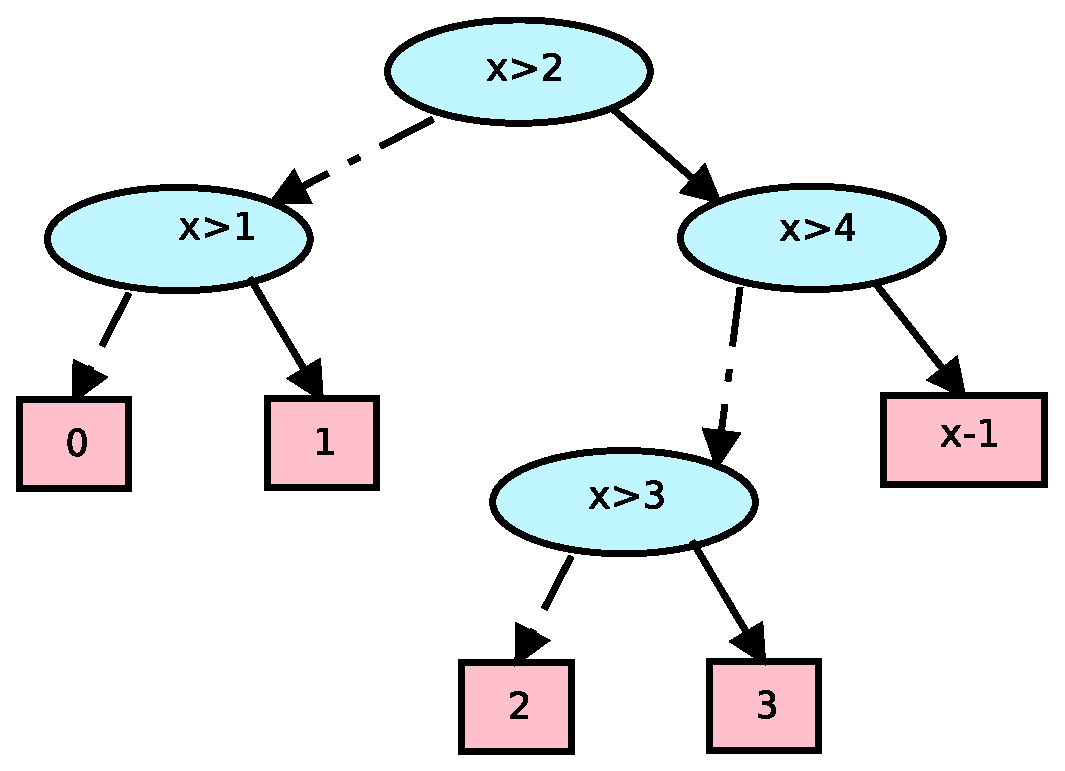
\includegraphics[scale=0.4]{Figures/xadds/samplexadd.eps} }
\caption{ Example of ADD.}
\label{fig:addapprox} 
\end{figure}
